\documentclass[12pt,letterpaper]{hmcpset}
\usepackage[margin=1in]{geometry}
\usepackage{graphicx}
\usepackage{amsthm}
\usepackage{enumitem}
\usepackage{hyperref}

% Theorems
\usepackage{amsthm}
\renewcommand\qedsymbol{$\blacksquare$}
\makeatletter
\@ifclassloaded{article}{
    \newtheorem{definition}{Definition}[section]
    \newtheorem{example}{Example}[section]
    \newtheorem{theorem}{Theorem}[section]
    \newtheorem{corollary}{Corollary}[theorem]
    \newtheorem{lemma}{Lemma}[theorem]
}{
}
\makeatother

% Random Stuff
\setlength\unitlength{1mm}

\newcommand{\insertfig}[3]{
\begin{figure}[htbp]\begin{center}\begin{picture}(120,90)
\put(0,-5){\includegraphics[width=12cm,height=9cm,clip=]{#1.eps}}\end{picture}\end{center}
\caption{#2}\label{#3}\end{figure}}

\newcommand{\insertxfig}[4]{
\begin{figure}[htbp]
\begin{center}
\leavevmode \centerline{\resizebox{#4\textwidth}{!}{\input
#1.pstex_t}}
\caption{#2} \label{#3}
\end{center}
\end{figure}}

\long\def\comment#1{}

\newcommand\norm[1]{\left\lVert#1\right\rVert}
\DeclareMathOperator*{\argmin}{arg\,min}
\DeclareMathOperator*{\argmax}{arg\,max}

% bb font symbols
\newfont{\bbb}{msbm10 scaled 700}
\newcommand{\CCC}{\mbox{\bbb C}}

\newfont{\bbf}{msbm10 scaled 1100}
\newcommand{\CC}{\mbox{\bbf C}}
\newcommand{\PP}{\mbox{\bbf P}}
\newcommand{\RR}{\mbox{\bbf R}}
\newcommand{\QQ}{\mbox{\bbf Q}}
\newcommand{\ZZ}{\mbox{\bbf Z}}
\renewcommand{\SS}{\mbox{\bbf S}}
\newcommand{\FF}{\mbox{\bbf F}}
\newcommand{\GG}{\mbox{\bbf G}}
\newcommand{\EE}{\mbox{\bbf E}}
\newcommand{\NN}{\mbox{\bbf N}}
\newcommand{\KK}{\mbox{\bbf K}}
\newcommand{\KL}{\mbox{\bbf KL}}

% Vectors
\renewcommand{\aa}{{\bf a}}
\newcommand{\bb}{{\bf b}}
\newcommand{\cc}{{\bf c}}
\newcommand{\dd}{{\bf d}}
\newcommand{\ee}{{\bf e}}
\newcommand{\ff}{{\bf f}}
\renewcommand{\gg}{{\bf g}}
\newcommand{\hh}{{\bf h}}
\newcommand{\ii}{{\bf i}}
\newcommand{\jj}{{\bf j}}
\newcommand{\kk}{{\bf k}}
\renewcommand{\ll}{{\bf l}}
\newcommand{\mm}{{\bf m}}
\newcommand{\nn}{{\bf n}}
\newcommand{\oo}{{\bf o}}
\newcommand{\pp}{{\bf p}}
\newcommand{\qq}{{\bf q}}
\newcommand{\rr}{{\bf r}}
\renewcommand{\ss}{{\bf s}}
\renewcommand{\tt}{{\bf t}}
\newcommand{\uu}{{\bf u}}
\newcommand{\ww}{{\bf w}}
\newcommand{\vv}{{\bf v}}
\newcommand{\xx}{{\bf x}}
\newcommand{\yy}{{\bf y}}
\newcommand{\zz}{{\bf z}}
\newcommand{\0}{{\bf 0}}
\newcommand{\1}{{\bf 1}}

% Matrices
\newcommand{\Ab}{{\bf A}}
\newcommand{\Bb}{{\bf B}}
\newcommand{\Cb}{{\bf C}}
\newcommand{\Db}{{\bf D}}
\newcommand{\Eb}{{\bf E}}
\newcommand{\Fb}{{\bf F}}
\newcommand{\Gb}{{\bf G}}
\newcommand{\Hb}{{\bf H}}
\newcommand{\Ib}{{\bf I}}
\newcommand{\Jb}{{\bf J}}
\newcommand{\Kb}{{\bf K}}
\newcommand{\Lb}{{\bf L}}
\newcommand{\Mb}{{\bf M}}
\newcommand{\Nb}{{\bf N}}
\newcommand{\Ob}{{\bf O}}
\newcommand{\Pb}{{\bf P}}
\newcommand{\Qb}{{\bf Q}}
\newcommand{\Rb}{{\bf R}}
\newcommand{\Sb}{{\bf S}}
\newcommand{\Tb}{{\bf T}}
\newcommand{\Ub}{{\bf U}}
\newcommand{\Wb}{{\bf W}}
\newcommand{\Vb}{{\bf V}}
\newcommand{\Xb}{{\bf X}}
\newcommand{\Yb}{{\bf Y}}
\newcommand{\Zb}{{\bf Z}}

% Calligraphic
\newcommand{\Ac}{{\cal A}}
\newcommand{\Bc}{{\cal B}}
\newcommand{\Cc}{{\cal C}}
\newcommand{\Dc}{{\cal D}}
\newcommand{\Ec}{{\cal E}}
\newcommand{\Fc}{{\cal F}}
\newcommand{\Gc}{{\cal G}}
\newcommand{\Hc}{{\cal H}}
\newcommand{\Ic}{{\cal I}}
\newcommand{\Jc}{{\cal J}}
\newcommand{\Kc}{{\cal K}}
\newcommand{\Lc}{{\cal L}}
\newcommand{\Mc}{{\cal M}}
\newcommand{\Nc}{{\cal N}}
\newcommand{\Oc}{{\cal O}}
\newcommand{\Pc}{{\cal P}}
\newcommand{\Qc}{{\cal Q}}
\newcommand{\Rc}{{\cal R}}
\newcommand{\Sc}{{\cal S}}
\newcommand{\Tc}{{\cal T}}
\newcommand{\Uc}{{\cal U}}
\newcommand{\Wc}{{\cal W}}
\newcommand{\Vc}{{\cal V}}
\newcommand{\Xc}{{\cal X}}
\newcommand{\Yc}{{\cal Y}}
\newcommand{\Zc}{{\cal Z}}

% Bold greek letters
\newcommand{\alphab}{\hbox{\boldmath$\alpha$}}
\newcommand{\betab}{\hbox{\boldmath$\beta$}}
\newcommand{\gammab}{\hbox{\boldmath$\gamma$}}
\newcommand{\deltab}{\hbox{\boldmath$\delta$}}
\newcommand{\etab}{\hbox{\boldmath$\eta$}}
\newcommand{\lambdab}{\hbox{\boldmath$\lambda$}}
\newcommand{\epsilonb}{\hbox{\boldmath$\epsilon$}}
\newcommand{\nub}{\hbox{\boldmath$\nu$}}
\newcommand{\mub}{\hbox{\boldmath$\mu$}}
\newcommand{\zetab}{\hbox{\boldmath$\zeta$}}
\newcommand{\phib}{\hbox{\boldmath$\phi$}}
\newcommand{\psib}{\hbox{\boldmath$\psi$}}
\newcommand{\thetab}{\hbox{\boldmath$\theta$}}
\newcommand{\taub}{\hbox{\boldmath$\tau$}}
\newcommand{\omegab}{\hbox{\boldmath$\omega$}}
\newcommand{\xib}{\hbox{\boldmath$\xi$}}
\newcommand{\sigmab}{\hbox{\boldmath$\sigma$}}
\newcommand{\pib}{\hbox{\boldmath$\pi$}}
\newcommand{\rhob}{\hbox{\boldmath$\rho$}}

\newcommand{\Gammab}{\hbox{\boldmath$\Gamma$}}
\newcommand{\Lambdab}{\hbox{\boldmath$\Lambda$}}
\newcommand{\Deltab}{\hbox{\boldmath$\Delta$}}
\newcommand{\Sigmab}{\hbox{\boldmath$\Sigma$}}
\newcommand{\Phib}{\hbox{\boldmath$\Phi$}}
\newcommand{\Pib}{\hbox{\boldmath$\Pi$}}
\newcommand{\Psib}{\hbox{\boldmath$\Psi$}}
\newcommand{\Thetab}{\hbox{\boldmath$\Theta$}}
\newcommand{\Omegab}{\hbox{\boldmath$\Omega$}}
\newcommand{\Xib}{\hbox{\boldmath$\Xi$}}

% mixed symbols
\newcommand{\sinc}{{\hbox{sinc}}}
\newcommand{\diag}{{\hbox{diag}}}
\renewcommand{\det}{{\hbox{det}}}
\newcommand{\trace}{{\hbox{tr}}}
\newcommand{\tr}{\trace}
\newcommand{\sign}{{\hbox{sign}}}
\renewcommand{\arg}{{\hbox{arg}}}
\newcommand{\var}{{\hbox{var}}}
\newcommand{\cov}{{\hbox{cov}}}
\renewcommand{\Re}{{\rm Re}}
\renewcommand{\Im}{{\rm Im}}
\newcommand{\eqdef}{\stackrel{\Delta}{=}}
\newcommand{\defines}{{\,\,\stackrel{\scriptscriptstyle \bigtriangleup}{=}\,\,}}
\newcommand{\<}{\left\langle}
\renewcommand{\>}{\right\rangle}
\newcommand{\Psf}{{\sf P}}
\newcommand{\T}{\top}
\newcommand{\m}[1]{\begin{bmatrix} #1 \end{bmatrix}}


% info for header block in upper right hand corner
\name{}
\class{Math189R SU20.1}
\assignment{Homework 1}
\duedate{Thursday, June 11, 2020}

\renewcommand{\labelenumi}{{(\alph{enumi})}}


\begin{document}

\begin{problem}[1]
(\textbf{Linear Transformation}) Let $\mathbf{y} = A\mathbf{x} + \mathbf{b}$ be a random vector.
show that expectation is linear:
\[
    \EE[\yy] = \EE[A\xx + \bb] = A\EE[\xx] + \bb.
\]
Also show that
\[
    \cov[\yy] = \cov[A\xx + \bb] = A \cov[\xx] A^\T = A\Sigmab A^\T.
\]
\end{problem}
\begin{solution}

  Expectation for a continuous random variable $x$ with normalized probability distribution function $f_x(x)$ is defined as

\[
  \EE[x]= \int_{-\infty}^{\infty} xf_X(x)dx
\]

  Consider first a single random variable $x$, and $y = ax + b$
\[
\EE[x] = \EE[ax + b]
         = \int_{-\infty}^{\infty} (ax + b) f_X(x) dx
         = a\int_{-\infty}^{\infty} x f_X(x) dx + b \int_{-\infty}^{\infty} f_X(x) dx
         = a\EE[x] + b
\]

In multiple variables, the $x_i$ are independent, so it follows that
\[
   \EE[A\xx + \bb] = A\EE[\xx] + \bb
\]

Covariance is defined
\[
  \CC[\xx] = \EE[(X - \EE[X])(X - \EE[X])^T]
\]

Again, since the expectation $\EE$ is linear in $\xx$, the covariance and any linear transformation of $\xx$ commute and can be rearranged.  The term in $\mathbf{b}$ vanishes because the covariance of a constant term is zero.
\[
  \yy = A\xx + \bb
\]

\[
  \CC(\yy) = \CC(A\xx + \bb)
           = A\CC(x)A^T
\]

Works used: \url{https://www.probabilitycourse.com/chapter6/6_1_5_random_vectors.php}

    \vfill
\end{solution}
\newpage




\begin{problem}[2]
Given the dataset $\Dc = \{(x,y)\} = \{(0,1), (2,3), (3,6), (4,8)\}$
\begin{enumerate}
   \item Find the least squares estimate $y = \thetab^\T\xx$ by hand using
        Cramer's Rule.
    \item Use the normal equations to find the same solution and verify it
        is the same as part (a).
    \item Plot the data and the optimal linear fit you found.
    \item Find randomly generate 100 points near the line with white Gaussian
        noise and then compute the least squares estimate (using a computer).
        Verify that this new line is close to the original and plot the new
        dataset, the old line, and the new line.
\end{enumerate}

\end{problem}
\begin{solution}
1. By Cramer's rule, we have the closed forms
\[
    m = \frac{n\sum_{i=1}^n x_iy_i - (\sum_{i=1}^n x_i)(\sum_{i=1}^n y_i)}{n\sum_{i=1}^n x_i^2 - (\sum_{i=1}^n x_i)^2}
\]
\[
    b = \frac{n\sum_{i=1}^n x_i^2y_i - (\sum_{i=1}^n x_i)(\sum_{i=1}^n x_iy_i)}{n\sum_{i=1}^n x_i^2 - (\sum_{i=1}^n x_i)^2}
\]
Evaluation gives
\[
\sum(x) = 9, \sum(y) = 18, \sum{x^2} = 29, \sum(xy) = 56, \sum(x^2y) = 194
\]
Then
\[
m = \frac{(4*56 - 9*18)}{4*29 - 81}
= \frac{62}{35} =~ 1.77
\]
and
\[
b = \frac{194}{35} =~ 5.54
\]

Numbers, on the other hand, finds $m = b = 1.2$ as the optimal fit.

2. Minimize the error $e$, where

\[
 e = \ee \cdot \ee
\]

\[
 \ee = \yy - ( m \xx + b )
\]

\[
 \ee =
 \begin{bmatrix}
   1 \\
   3 \\
   6 \\
   8 \\
\end{bmatrix}
 - m *
\begin{bmatrix}
  0 \\
  2 \\
  3 \\
  4 \\
\end{bmatrix}
 - b
\]

\[
 \ee =
 \begin{bmatrix}
   1 - b\\
   3 - 2m - b\\
   6 - 3m - b\\
   8 - 4m - b\\
\end{bmatrix}
 \]

\[
e = (1-b)^2 + (3 - 2m - b)^2 + (6 - 3m - b)^2 + (8 - 4m - b)^2
\]

Then find
\[
\begin{aligned}
\frac{\partial e}{\partial m} & = -2m[(3 - 2m - b) + (6 - 3m - b) + (8 - 4m - b)] \\
& = -2(17 - 9m - 3b)
\end{aligned}
\]

\[
\begin{aligned}
\frac{\partial e}{\partial b} & = -2b[(1-b) + (3 - 2m - b) + (6 - 3m - b) + (8 - 4m - b)] \\
& = -2(18 - 9m - 4b)
\end{aligned}
 \]

Used Mathematica to solve this system, with result
\[
  m = \frac{14/9}, b = 1
\]

 3. Attached graph produced by Numbers.

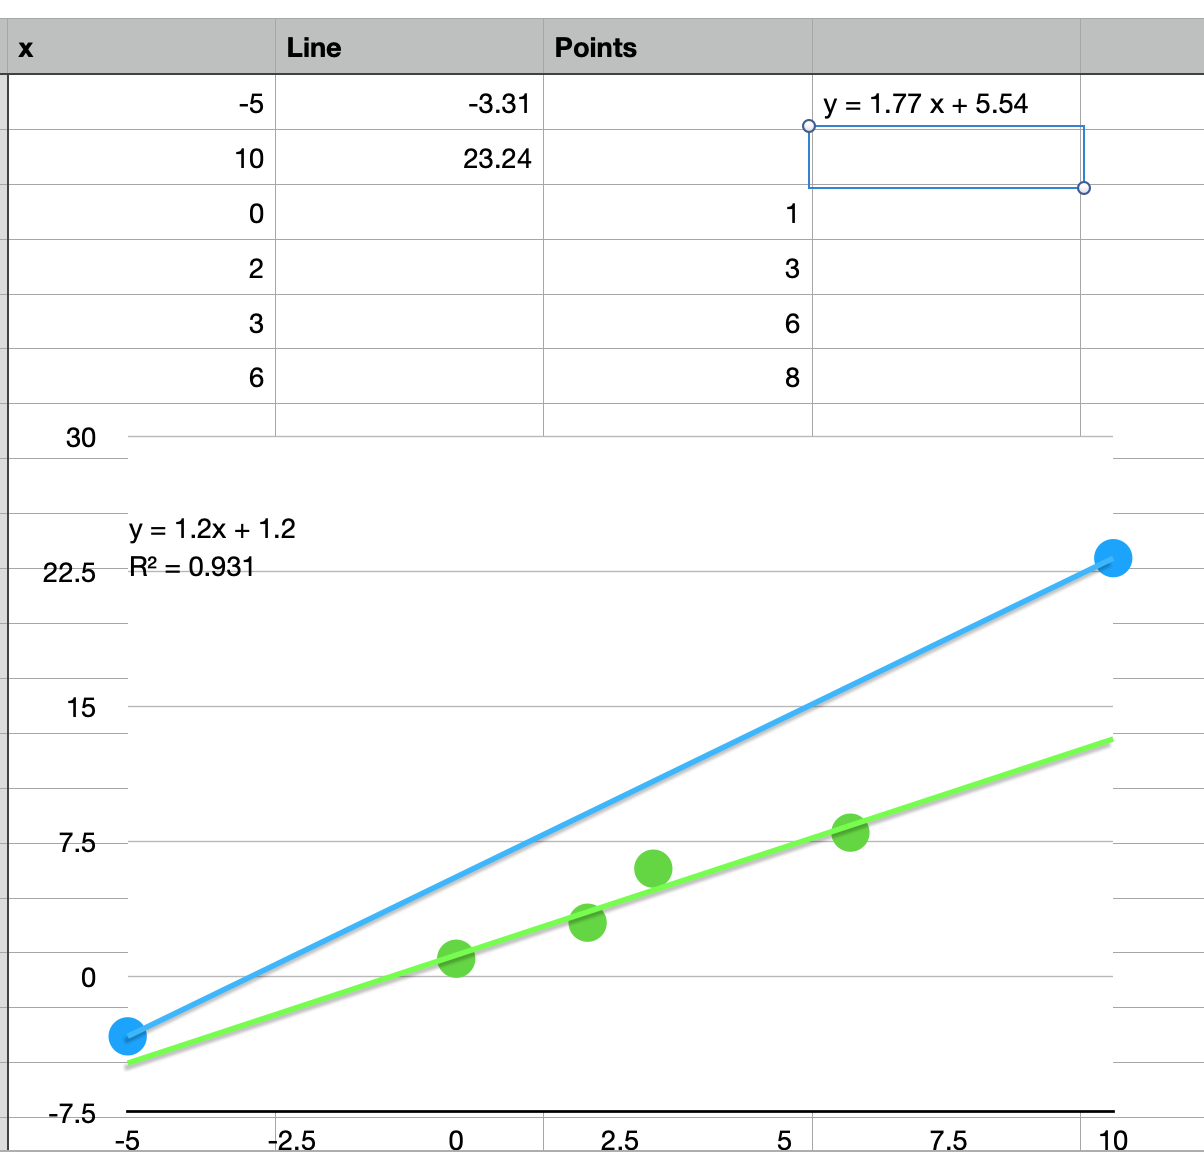
\includegraphics[scale=0.4]{hw1-p2-graph1.png}

\newpage

4. Using $(m,b) = (1.2, 1.2)$

Generated 100 gaussian random numbers (mean = 0.0, variance = 1.0) from \url{https://www.random.org/gaussian-distributions/?num=100&mean=0.0&stdev=0.5&dec=3&col=1&notation=scientific&format=html&rnd=new}

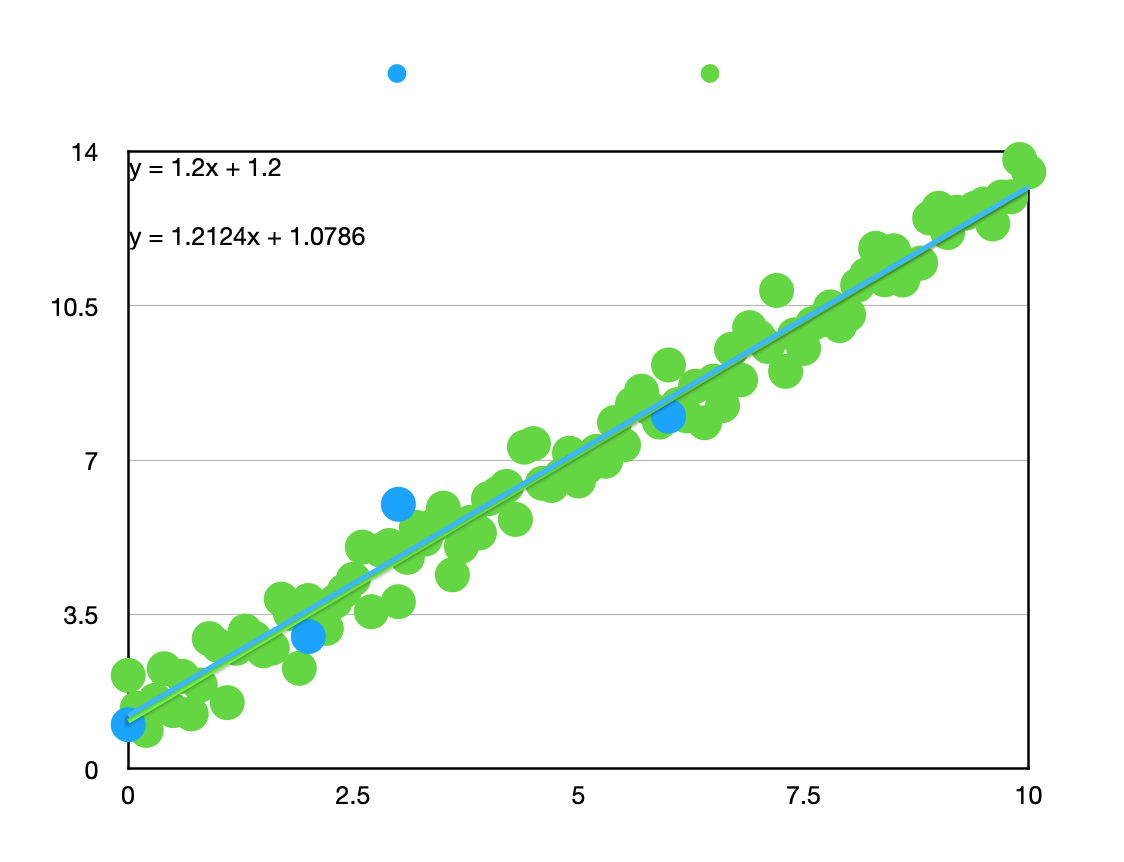
\includegraphics[scale=0.4]{hw1-p2-graph2.png}

(Data exported in csv format in git repository.)


    \vfill
\end{solution}
\newpage



\end{document}
